\documentclass[11pt]{standalone}
\usepackage{amssymb}
\usepackage{amsmath}
\usepackage[no-math]{fontspec}
\usepackage{unicode-math}
\usepackage{libertinus}
\usepackage{pgf,xcolor}
\usepackage{tikz}
\usetikzlibrary{arrows.meta, backgrounds}
\usepackage{pgfplots}
\pgfplotsset{compat=newest}

\definecolor{my_darkgray}{HTML}{484949}
\definecolor{my_lightgray}{HTML}{F3F4F4}
\definecolor{my_darkblue}{HTML}{005A94}
\definecolor{my_lightblue}{HTML}{CCDEE9}
\definecolor{my_yellow}{HTML}{FFEC7F}
\definecolor{my_red}{HTML}{E60000}
\definecolor{my_orange}{HTML}{E87846}

\begin{document}
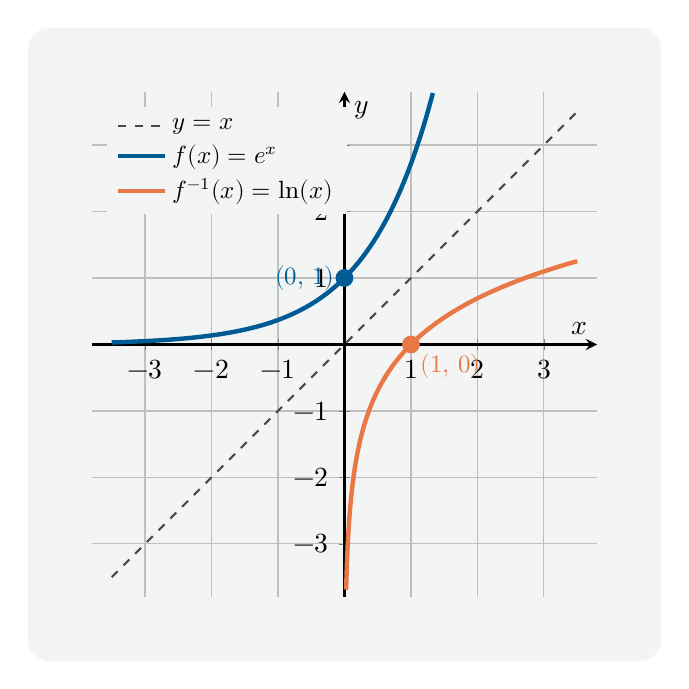
\begin{tikzpicture}[
    show background rectangle,
    background rectangle/.style={fill=my_lightgray, rounded corners=8pt},
    inner frame sep=0.8cm
]
\begin{axis}[
    axis lines=center,
    xlabel={$x$},
    ylabel={$y$},
    height=8cm, width=8cm,
    xmin=-3.8, xmax=3.8,
    ymin=-3.8, ymax=3.8,
    xtick={-3,-2,-1,0,1,2,3},
    ytick={-3,-2,-1,0,1,2,3},
    grid=both,
    axis equal,
    axis line style={thick},
    clip=true,
    legend style={
        font=\small,
        at={(0.03, 0.97)},
        anchor=north west,
        draw=none,
        fill=my_lightgray,
    },
    legend cell align=left,
]

% Mirror line y = x (dashed, my_darkgray)
\addplot[draw=my_darkgray, dashed, thick, domain=-3.5:3.5]{x};
\addlegendentry{$y = x$}

% e^x (my_darkblue): only plot where it stays within the window
% e^x = 3.8 at x = ln(3.8) ~ 1.335; e^x > 0 always.
\addplot[draw=my_darkblue, samples=300, ultra thick, domain=-3.5:1.33]
    {exp(x)};
\addlegendentry{$f(x)=e^x$}

% ln(x) (my_orange): defined only for x > 0
% ln(3.8) ~ 1.335; the curve exits the bottom at x = e^{-3.8} ~ 0.022.
\addplot[draw=my_orange, samples=300, ultra thick, domain=0.025:3.5]
    {ln(x)};
\addlegendentry{$f^{-1}(x)=\ln(x)$}

% Shared point (1, 0) on ln(x) and (0, 1) on e^x are already on the curves.
% Mark the point (1,1) which lies on y=x and is the "equal" crossing.
% (e^1 = e ≠ 1, so (1,1) is NOT on e^x — no special marker needed there.)

% Mark the zero of ln: (1, 0)
\addplot[only marks, mark=*, mark size=3pt,
         draw=my_orange, fill=my_orange]
    coordinates{(1, 0)};
\node[below right, font=\small, my_orange] at (axis cs:1, 0) {$(1,\,0)$};

% Mark the y-intercept of e^x: (0, 1)
\addplot[only marks, mark=*, mark size=3pt,
         draw=my_darkblue, fill=my_darkblue]
    coordinates{(0, 1)};
\node[left, font=\small, my_darkblue] at (axis cs:0, 1) {$(0,\,1)$};

% Vertical asymptote hint: ln(x) -> -inf as x -> 0+
% A short dashed line along x=0 from y=-3.5 upward is already the y-axis,
% so no extra element is needed.

\end{axis}
\end{tikzpicture}
\end{document}
